
\chapter{Konvergence na prostoru náhodných veličin}
\begin{define}
	Mějme $(X_n)_{n=1}^{+\infty}$ na $\LL_p$, případně $\L_p\prostor$. Definujeme $X_n\stackrel{\L_p}{\longrightarrow} X$, pokud\newline $\left\| X_n-X\right\| \to 0$,  $\left\| X_n-X\right\|_{\L_p}^p=\E \left[ |X_n-X|^p \right]$.
\end{define}
\begin{remark}
	Pro vektorové náhodné veličiny $\X_n,~\X$ do $\R^s$ platí, že
	$$|\X_n-\X|=\left\|\X_n-\X\right\|_\epsilon = \sqrt{\sum\limits_{n=1}^s \br{ X_n^i(\omega)-X^i(\omega)}^2},$$ kde $\left\| \right\|_\epsilon$ označuje Euklidovskou normu.
\end{remark}
\begin{theorem}
	Nechť $1\leq p\leq q\leq +\infty$. Pak na $\prostor$ platí, že $$\LL_q\subset \LL_p\text{ a }X_n\stackrel{\L_q}{\longrightarrow}X~\Rightarrow~ X_n\stackrel{\L_p}{\longrightarrow}X.$$ 
\end{theorem}
\begin{remark}
	\begin{enumerate}
		\item Implikaci nelze obrátit. 
		\item $q>p~\Rightarrow~$ topologie $\L_q$ je silnějí než topologie $\L_p$.
	\end{enumerate}
\end{remark}
\begin{define}
	Mějme $\posln$ náhodné veličiny na $\prostor$. Pak definujeme \textbf{konvergenci s.j.} jako $X_n\stackrel{s.j.~(\PP)}{\longrightarrow}X$, pokud $\PP\{ \omega:X_n(\omega)\to X(\omega) \}=1$.
\end{define}
\begin{remark}
	$X_n\Lp X $ není ekvivalentní s $ X_n\sj X$.
\end{remark}
\begin{theorem}
	\[
	\begin{split}
	X_n\sj X&\Leftrightarrow(\forall\epsilon>0)\biggl( \lim\limits_{ k\to +\infty} \PP\Bigl( \bigcup\limits_{n\geq k}\{\omega:\left| X_n(\omega)-X(\omega) \right|\geq \epsilon\} \Bigr)=0\biggr) \\
	&\Leftrightarrow(\forall\epsilon>0)\biggl( \lim\limits_{ k\to +\infty} \PP\Bigl( \bigcap\limits_{n\geq k}\{\omega:\left| X_n(\omega)-X(\omega) \right|< \epsilon\} \Bigr)=1\biggr)
	\end{split}
	\]
	\begin{proof}
		\[
		\begin{split}
		X_n\sj X~&\Leftrightarrow~\PP\left( \lim\limits_{ n\to +\infty}X_n(\omega)=X(\omega) \right)=\PP\biggl( \omega: (\forall\epsilon>0)(\forall n\geq k)\bigl(|X_n-X|<\epsilon\bigr) \biggr) = \\
		&=~\PP\left( \bigcap\limits_{\epsilon>0}\bigcup\limits_{k\geq 1}\bigcap\limits_{n\geq k}\{ \omega: |X_n-X|<\epsilon \} \right)=1
		\end{split}
		\] 
		$$ \PP\biggl(\bigcup\limits_{k\geq 1}\underbrace{ \bigcap\limits_{n\geq k}\{ \omega: |X_n-X|<\epsilon}_{A_k^\epsilon\nearrow A^\epsilon=\bigcup A_k^\epsilon} \} \biggr)=1 ~~~\forall\epsilon>0$$
		$\PP$ je spojitá zdola: $ A_n\nearrow A=\bigcup A_n ~\Rightarrow~\lim\limits_{ n\to +\infty}\PP(A_n)=\PP(A) $,~~tedy
		$$\lim\limits_{ k\to +\infty}\PP\Bigl( \bigcap\limits_{n\geq k}\{\omega: |X_n-X|<\epsilon \} \Bigr)=1~~~\forall\epsilon>0.$$
		
	\end{proof}
\end{theorem}
\begin{dusl}
	$$ X_n\sj X~\Rightarrow~ \PP\bigl( \{\omega: |X_n-X|\geq\epsilon \} \bigr)\to 0~~~\forall\epsilon>0 $$\begin{proof}
		$$ X_n\sj X \Rightarrow \underbrace{\PP\Bigl( \bigcup\limits_{n\geq k}\{\omega: |X_n-X|\geq\epsilon \} \Bigr)}_{\to0}\geq \PP\bigl( \{\omega: |X_k-X|\geq \epsilon \} \bigr)\geq 0~~~\forall\epsilon>0. $$
	\end{proof}
\end{dusl}
\begin{define}
	Mějme $(X_n)_{n=1}^{+\infty}$. Pak definujeme \textbf{konvergenci podle $\PP$}, ozn. $X_n\stackrel{\PP}{\to}X$, jako 
$$
	(\forall\epsilon>0)\Bigl(\PP\left( |X_n-X|\geq \epsilon \right)\to0\Bigr)~~\Leftrightarrow~~(\forall\epsilon>0)\Bigl(\PP\left( |X_n-X|< \epsilon \right)\to1\Bigr).
$$
\end{define}
\begin{theorem}
	 $X_n\sj X~\Rightarrow~ X_n\stackrel{\PP}{\to}X$ (nelze obrátit)
\end{theorem}
\begin{theorem}
	$$ X_n\stackrel{\PP}{\to}X \Leftrightarrow \lim\limits_{ n\to +\infty}\E \underbrace{\left( \frac{|X_n-X|}{1+|X_n-X|} \right)}_{\rho(X_n,X)}=0, $$
	kde $\rho(x,y)=\frac{|x-y|}{1+|x-y|}$ je metrika.
	\begin{proof}
		\begin{enumerate}[$\Rightarrow:$]
			\item BÚNO: $X=0~ s.j.$, protože $X_n\stackrel{\PP}{\to}X \Leftrightarrow X_n-X\stackrel{\PP}{\to}0$ (potom by stačilo použít $Y_n:=X_n-X$). Zkoumáme tedy, jestli platí následující rovnost:
			\[
			\begin{split}
			&X_n\stackrel{\PP}{\to}0\stackrel{?}{\Rightarrow} \lim\limits_{ n\to +\infty} \E \left( \frac{|X_n|}{1+|X_n|}\right)=0 \\
			0\leq \E \left( \frac{|X_n|}{1+|X_n|} \right)&=\int\limits_{\Omega}\frac{|X_n|}{1+|X_n|}\dif\PP\equal{\text{fixní}~\epsilon}\int\limits_{\{ \omega:|X_n|\geq\epsilon \}}\underbrace{\frac{|X_n|}{1+|X_n|}}_{\leq 1}\dif\PP+\int\limits_{\{ \omega:|X_n|<\epsilon \}}\underbrace{\frac{|X_n|}{1+|X_n|}}_{<\epsilon}\dif\PP\leq \\
			&\leq \PP(\omega:|X_n|\geq \epsilon)+\int\limits_{\{ |X_n|<\epsilon \}}\epsilon \dif\PP\leq \underbrace{\PP(|X_n|\geq \epsilon)}_{\to 0\text{ pro }n\to+\infty}+~\epsilon\cdot 1~~~~~\forall\epsilon>0\end{split}\]
		\end{enumerate}
	\begin{enumerate}[$\Leftarrow:$]
		\item 	$$\lim\limits_{ n\to +\infty} \E \underbrace{\left( \frac{|X_n-X|}{1+|X_n-X|} \right)}_{\leq 1\in\LL_1\prostor}\equal{\text{LDCT}}\E \underbrace{\left( \lim\limits_{ n\to +\infty}\frac{|X_n-X|}{1+|X_n-X|} \right)}_{Y\geq 0}=0,
		$$	tzn. $\E Y=0$, kde $Y\geq 0$. Pak $Y=0~s.j.~\PP$, tedy
		$ \PP\left( \lim\limits_{ n\to +\infty}\frac{|X_n-X|}{1+|X_n-X|}=0 \right)=1, $
		z čehož vyplývá, že $$ \frac{|X_n-X|}{1+|X_n-X|} \sj 0~\Rightarrow~|X_n-X|\sj 0~\Rightarrow~ X_n\sj X~\Rightarrow~ X_n\stackrel{\PP}{\to}X $$
	\end{enumerate}
	\end{proof}
\end{theorem}
\begin{lemma}
	$X_n\Lp X~\Rightarrow~ X_n\Pto X$
	\begin{proof}[Důkaz pro $p=1$]
		 Markov (Čebyšev) na $\L_1$: $(\forall\epsilon>0)\Bigl(\PP(|X|\geq \epsilon)\leq \frac{\E |X|}{\epsilon}\Bigr)$.
		Za $|X|$ nyní dosadíme $ |X_n-X| $.
		$$ 0\leq \PP\br{|X_n-X|\geq \epsilon}\leq \frac{\E |X_n-X|}{\epsilon}=\frac{\left\| X_n-X\right\|_{\L_1}}{\epsilon}\to 0 ~~~\forall\epsilon>0 $$
	\end{proof}
\end{lemma}
\begin{theorem}\label{podposloupnost}
	$X_n\Pto X~\Rightarrow~ \exists (n_k)_{k=1}^{+\infty}$ tak, že $X_{n_k}\sj X$.
	\begin{proof}
		\[
		\begin{split}
		\lim\limits_{ n\to +\infty}\E \left( \frac{|X_n-X|}{1+|X_n-X|} \right)=0~&\Rightarrow~\exists n_k:~~\E \left( \frac{|X_{n_k}-X|}{1+|X_{n_k}-X|} \right)\leq \frac{1}{2^k}~\Rightarrow \\
		&\Rightarrow~\sum\limits_{k=1}^{+\infty}\E \left( \frac{|X_{n_k}-X|}{1+|X_{n_k}-X|} \right)\leq \sum\limits_{k=1}^{+\infty}\frac{1}{2^k}=1<+\infty
		\end{split}
		\] 
		dle MCT:
		$$ \E \Bigl( \sum\limits_{k=1}^{+\infty}\frac{|X_{n_k}-X|}{1+|X_{n_k}-X|} \Bigr)<+\infty~\Rightarrow~ \sum\limits_{k=1}^{+\infty}\frac{|X_{n_k}-X|}{1+|X_{n_k}-X|}<+\infty~~s.j.~\PP $$
		Tedy nutná podmínka (z kritéria konvergence řady): $$ \frac{|X_{n_k}-X|}{1+|X_{n_k}-X|}\sj 0~~~\Rightarrow~~~|X_{n_k}-X|\sj0 $$
	\end{proof}
\end{theorem}
\begin{theorem}[LDCT podle $\PP$]
	Nechť $X_n\Pto X$ a $(\forall n\in\N)\Bigl(|X_n|\stackrel{s.j.}{\leq}Y\in\LL_{p\geq 1}\Bigr)$.\newline Pak $X\in\LL_p$ a $X_n\Lp X$. 
	\begin{proof}
		~\begin{enumerate}[	a)]
			\item $X_n\Pto X$ a $|X_n|\stackrel{s.j.}{\leq}Y~\Rightarrow~ |X|\stackrel{s.j.}{\leq}Y$
			\item Spor: nechť \textbf{neplatí} $X_n\Lp X$, tzn. $\exists (n_k)_{k=1}^{+\infty}$ vybraná tak, že  $\E \left| X_{n_k}-X \right|^p>\epsilon$. Potom
			\[
			\begin{split}
			X_n\Pto X~&\Rightarrow~ X_{n_k}\Pto X~\stackrel{\ref{podposloupnost}}{\Longrightarrow}~ \exists X_{n_{k_j}}\sj X~\Rightarrow~\\ &\Rightarrow~ \lim\limits_{ j\to +\infty} \E \bigl|X_{n_{k_j}}-X\bigr|^p\equal{\text{LDCT}} \E  \Br{\lim\limits_{ j\to +\infty}\bigl| X_{n_{k_j}}-X \bigr|^p }=\E (0_{s.j.})=0,
			\end{split}
			\] protože 
			$$ |X_{n_{k_j}}-X|\leq \left| X_{n_{k_j}} \right|+|X|\leq Y+Y=2Y\in\LL_p $$
		
		\end{enumerate}
	\end{proof}
\end{theorem}

\begin{theorem}
	Mějme $(\X_n)_{n=1}^{+\infty}$ do $\R^s$, $g:\R^s\to\R^1$ borelovsky měřitelnou a spojitou $s.j.~\PP^\X$. Potom \[
	\begin{split}
	\X_n\sj \X~~&\Rightarrow~~g(\X_n)\sj g(\X)\text{, tedy~~~}g\circ \X_n \sj g\circ X \\
	\X_n\Pto \X~~&\Rightarrow~~g(\X_n)\Pto g(\X)\text{, tedy~~~}g\circ \X_n \Pto g\circ \X.
	\end{split}
	\]	
	\begin{proof}
		\begin{enumerate}[	a)]
			\item $\sj$: Ponecháno čtenáři.
			\item $\Pto$: Sporem: nechť $g(\X_n)\stackrel{\PP}{\nrightarrow}g(\X)$, tedy $\exists (n_k)_{k=1}^{+\infty}$~~tak, že~~$\PP\left( \left| g(\X_{n_k})-g(\X) \right|\geq \epsilon \right)>\delta$.
			\[
			\begin{split}
			\text{Z předpokladu~~}\Bigl(\X_{n_k}\Bigr)_{k=1}^{+\infty}\Pto \X~&\stackrel{\ref{podposloupnost}}{\Longrightarrow}~\exists \left( \X_{n_{k_j}} \right)_{j=1}^{+\infty}\text{ tak, že }\X_{n_{k_j}}\sj \X \stackrel{dle~a)}{~\Longrightarrow~}\\ &\Rightarrow~g\left( \X_{n_{k_j}} \right)\sj g(\X)~\Rightarrow~ g\left( \X_{n_{k_j}} \right)\Pto g(\X) \text{ (spor)} 
			\end{split}
			\]  
		\end{enumerate}
	\end{proof}
\end{theorem}
\begin{dusl}
	 Mějme $X_n\Pto X$ a $Y_n \Pto Y$, $g:\R^2\to\R^1$ měřitelnou spojitou $s.j.~\PP^{(X,Y)}$. Pak $g(X_n,Y_n)\Pto g(X,Y)$ \begin{proof}
		$X_n\Pto X\text{ a }Y_n \Pto Y\Leftrightarrow (X_n,Y_n)\Pto (X,Y)\stackrel{g~spoj.~s.j.}{\Longrightarrow}g(X_n,Y_n)\Pto g(X,Y)$
	\end{proof}
\end{dusl}
\begin{dusl}
	$$ X_n\Pto X\text{ a }Y_n \Pto Y ~\Rightarrow~ X_n+Y_n\Pto X+Y $$
\end{dusl}





\chapter{Limitní věty - Zákony velkých čísel (Laws of Large Numbers)}
Domluva: Mějme náhodné veličiny $\posln$ na $\prostor$, označme $S_n:=\sum\limits_{j=1}^n X_j$, $\oxn:=\frac{S_n}{n} $,
\[
\begin{split}
X_j\in\LL_1 &~~~\Rightarrow~~~ \E X_j\equal{ozn}\mu_j,~~\omn\equal{ozn}\frac{1}{n}\sum\limits_{j=1}^n \mu_j \\
X_j\in\LL_2 &~~~\Rightarrow~~~ \D X_j\equal{ozn}\sigma_j^2,~~\osn =\frac{1}{n}\sum\limits_{j=1}^n \sigma_j^2 \\
X_j\in\LL_1&\stackrel{iid}{~~~\Rightarrow~~~}\E X_j=\mu_j=\mu~~~\Rightarrow~~~\omn =\mu \\
X_j\in\LL_2&\stackrel{iid}{~~~\Rightarrow~~~}\D X_j=\sigma_j^2=\sigma^2~~\Rightarrow~~~\osn =\sigma^2
\end{split}
\] 
\begin{theorem}[Čebyševova, SlZVČ]
	Nechť $\posl\in\LL_2$ jsou po dvou nezávislé. Pak platí
	$$\sup\limits_{j\in\N}\D X_j = \sup\limits_{j\in\N}\sigma_j^2<+\infty~~~\Rightarrow~~~\oxn  - \omn \Pto 0.$$\begin{proof}
		\[
		\begin{split}
		\E \oxn &=\frac{1}{n}\sum\limits_{j=1}^n \E X_j=\frac{1}{n}\sum\limits_{j=1}^n \mu_j=\omn  \\
		\D \oxn &=\frac{1}{n^2}\D \Bigl(\sum\limits_{j=1}^n X_j\Bigr)\equal{\ref{Decko}}\frac{1}{n^2}\Bigl[\sum\limits_{j=1}^n \D X_j+\sum\limits_{i\neq j}\underbrace{\Cov(X_i,X_j)}_{=0}\Bigr]=\frac{1}{n}\osn  
		\end{split}
		\]	
		Čebyševova nerovnost na $\LL_2$: (pro zopakování)
		$$ X\in\LL_2~~~\Rightarrow~~~
		(\forall\epsilon>0)\Bigl( \PP\bigl( |X-\E X|\geq\epsilon \bigr)\leq \frac{\D X}{\epsilon^2} \Bigr)	  $$
		Nyní dosadíme za $X$ veličinu $\oxn $. Tvrzení pak vyplývá z definice konvergence podle $\PP$.
		$$	
		(\forall\epsilon>0)\Bigl( \PP\bigl( |\oxn -\omn |\geq\epsilon \bigr)\leq \frac{\osn }{n\epsilon^2}\leq \frac{K}{n\epsilon^2}\stackrel{n\to+\infty}{\longrightarrow}0 \Bigr)$$
	\end{proof}
\end{theorem}
\begin{remark}
	SlZVČ je zkratka pro "Slabý zákon velkých čísel", anglicky "Weak Law of Large Numbers".
\end{remark}
\begin{remark}
	V praxi používáme tuto verzi: $$ (\forall\epsilon>0)\Bigl( \PP\bigl(|\oxn-\omn|<\epsilon\bigr)\geq 1-\frac{K}{n\epsilon^2} \Bigr) $$
\end{remark}
\begin{dusl}
	Pokud existuje $\lim\limits_{ n\to +\infty}\omn\equal{\text{ozn}}m\in\R$, pak $\oxn\Pto m$.
\end{dusl}
\begin{theorem}[Standardní SlZVČ]
	Mějme $\posl\in \LL_2~iid$. Pak $\oxn \Pto \mu=\E X_j~~\forall j\in\N$, tzn. $(\forall\epsilon>0)\Bigl( \PP(|\oxn-\mu|<\epsilon)\to 1 \Bigr)$. 
\end{theorem}
\begin{theorem}[Bernoulliho SlZVČ]
	Mějme $\posl\stackrel{id}{\sim} \mathrm{A}(p)$, tedy $$ X_j=\begin{cases}
	1 & \text{s pravděpodobností }p\in(0,1) \\ 0 & \text{s pravděpodobností }1-p=q 
	\end{cases},~~p=\PP(B)~(\text{jevu}~B),~\E X_j=p,~\D X_j=pq ,$$
	pak $$ \oxn=\parunderbrace{\frac{S_n}{n}}{\text{Relativní četnost výskytu jevu B}}\Pto p=\PP(B) $$
	a po dosazení do Čebyševovy nerovnosti: 
	$$  (\forall\epsilon>0)\Biggl( \PP\Bigl( \left|\frac{S_n}{n}-p \right|<\epsilon \Bigr)\geq 1-\frac{p(1-p)}{n\epsilon^2} \Biggr) $$
\end{theorem}
\begin{remark}
	$\mathrm{A}(p)$ je Kůsovo značení Bernoulliho rozdělení (a nazývá ho asymetrické rozdělení).
\end{remark}
\begin{theorem}[Standardní SiZVČ]
	Mějme $\posl~iid~\LL_2$. Pak $\oxn\sj\mu$, tzn.\newline $\PP\Bigl( \{ \omega:\lim\limits_{ n\to +\infty}\oxn(\omega)=\mu \} \Bigr)=1$.
\end{theorem}
\begin{theorem}[Borel. SiZVČ]
	Mějme nezávislé $\posl\sim \mathrm{A}(p)$. Pak $\oxn\sj p=\PP(B)$.
\end{theorem}
\begin{lemma}[Kolmogorovova nerovnost] \label{kolmner}
	Mějme vzájemně nezávislé $\posl\in\LL_2,$\newline$\E X_j=0$. Pak\newline $$(\forall\epsilon>0)\biggl( \PP\Br{\max\limits_{k\leq n}|S_k|\geq\epsilon}\leq \frac{\D S_n}{\epsilon^2}=\frac{\E S_n^2}{\epsilon^2}-\underbrace{\frac{(\E S_n)^2}{\epsilon^2}}_{=0} \biggr).$$
	\begin{proof}
		Definujeme $$ \xi_k=\begin{cases}
		1 &(\forall j\in\widehat{k-1})(|S_j|<\epsilon)\text{ a }|S_k|\geq \epsilon \\ 0 &\text{jinak}
		\end{cases}~\Rightarrow~\suminftyk\xi_k=\begin{cases}
		1 &\text{došlo alespoň k 1 překročení }\geq \epsilon\\0 &\text{nedošlo k žádnému překročení}
		\end{cases} $$
		\[
		\begin{split}
		\E S_n^2 &\geq \E \Bigl( \suminftykn\xi_k S_n^2 \Bigr)=\E \Bigl( \suminftykn\xi_k \bigl(S_k+(S_n-S_k)\bigr)^2 \Bigr)= \\ 
		&= \E \Bigl[ \suminftykn\xi_k S_k^2 +2\suminftykn\xi_k S_k(S_n-S_k)+\suminftykn\xi_k(S_n-S_k)^2 \Bigr]\geq \E \Bigl[ \suminftykn\xi_k S_k^2 +2\suminftykn\xi_k S_k(S_n-S_k) \Bigr]= \\ 
		&=
		\E \Bigl( \suminftykn\xi_k S_k^2\Bigr) +2\suminftykn \E \Bigl(\xi_k S_k(S_n-S_k) \Bigr)\equal{*}	\E \Bigl( \suminftykn\xi_k S_k^2\Bigr)+2\suminftykn \E (\xi_k S_k)\underbrace{\E (S_n-S_k)}_{=0} = \\ 
		&= 
		\E \Bigl( \suminftykn\xi_k S_k^2\Bigr)\stackrel{\forall k\in\hat{n}}{\geq} \E \Bigl( \suminftykn\xi_k \epsilon^2\Bigr)=\epsilon^2 \E \Bigl( \suminftykn\xi_k \Bigr)=\epsilon^2 \int\limits_{\Omega} \suminftykn\xi_k\dif\PP=\epsilon^2\int\limits_{\{ \omega:\suminftykn\xi_k=1 \}}1\dif\PP=\\ 
		&= \epsilon^2 \PP\Bigl( \suminftykn\xi_k=1 \Bigr)=\epsilon^2 \PP\Bigl( \max\limits_{k\leq n}|S_k|\geq \epsilon \Bigr)
		\end{split}
		\]
		($\ast $) ~ $\xi_k S_k$ závisí pouze na $X_1,...,X_k$ ~a~ $(S_n-S_k)=\sum\limits_{j=k+1}^nX_j$ závisí pouze na $X_{k+1},...,X_n$, kde $\E X_j=0$ (z předpokladu) a $X_j$ jsou nezávislé,
		tedy $\E (S_n-S_k)=0$.
	\end{proof}
\end{lemma}
\begin{theorem}[Kolmogorov 1 - SiZVČ]
	Mějme vzájemně nezávislé $\posl\in\LL_2$. Potom platí
	$$\suminfty\frac{\sigma_j^2}{j^2}<+\infty~~~\Rightarrow~~~\oxn-\omn\sj 0.$$
		\begin{proof}
		BÚNO: $(\forall j\in\N)(\E X_j=0)\Rightarrow\omn=0$. Pokud $\E X_j\neq 0$, pak použijeme $X'_j=X_j-\mu_j$. 
		Definujeme nyní $Y_m:=\max\limits_{k\leq 2^m}|S_k|$. Pak platí, že 
		$$ |\oxn|= \left| \frac{S_n}{n} \right|\leq\frac{Y_m}{2^{m-1}}=2\cdot\frac{Y_m}{2^m}~~~\forall n\in[2^{m-1},2^m] $$
		\[
		\begin{split}
		\suminftym \PP\Bigl( \frac{Y_m}{2^m}\geq \epsilon \Bigr)&=\suminftym \PP\Bigl( Y_m\geq \underbrace{\epsilon\cdot 2^m}_{\epsilon'} \Bigr)\stackrel{\ref{kolmner}}{\leq}\suminftym\frac{\E S_{2^m}^{~2}}{\epsilon^2\cdot4^m}=\frac{1}{\epsilon^2}\suminftym\frac{1}{4^m}\sum\limits_{k=1}^{2^m}\sigma_k^2= \\ &=\begin{array}{|l|}
		\text{Kroneckerovo}\\\text{přerovnání}		
		\end{array}\leq \frac{1}{\epsilon^2}\suminftyk \sigma_k^2\sum\limits_{m:2^m\geq k}^{+\infty}\frac{1}{4^m}=\frac{1}{\epsilon^2}\suminftyk \sigma_k^2\frac{1}{k^2}\frac{1}{1-\frac{1}{4}}= \\ &=\frac{4}{3}\frac{1}{\epsilon^2}\suminftyk \frac{\sigma_k^2}{k^2}<+\infty~~~\forall\epsilon>0  
		\end{split}
		\] 
	Z toho vyplývá, že řada zbytků 
	$$ \sum\limits_{m\geq k}^{+\infty} \PP\Bigl( \frac{Y_m}{2^m}\geq \epsilon \Bigr)\stackrel{k\to+\infty}{\longrightarrow}0\text{ a zároveň }\sum\limits_{m\geq k}^{+\infty} \PP\Bigl( \frac{Y_m}{2^m}\geq \epsilon \Bigr)\geq  \PP\biggl(\bigcup\limits_{m\geq k}^{+\infty} \Bigl(\frac{Y_m}{2^m}\geq \epsilon \Bigr)\biggr). $$
	$$ \text{A proto~~~}\PP\biggl(\bigcup\limits_{m\geq k}^{+\infty} \Bigl(\frac{Y_m}{2^m}\geq \epsilon \Bigr)\biggr)\stackrel{k\to+\infty}{\longrightarrow}0~~~\Rightarrow~~~\frac{Y_m}{2^m}\sj0~~~\Rightarrow~~~\oxn\sj0 $$
	\end{proof}
\end{theorem}
\begin{remark}
	SiZVČ je zkratka pro "Silný zákon velkých čísel", anglicky "Strong Law of Large Numbers".
\end{remark}
\begin{remark}
	Z Kolmogorovovy věty přímo vyplývá Čebyševova věta. \begin{proof}
		$$ \sup\limits_{j\in\N} \sigma_j^2\leq K~\Rightarrow~ \suminfty \frac{\sigma_j^2}{j^2}\leq K\suminfty \frac{1}{j^2}<+\infty~\Rightarrow~\oxn-\omn\sj 0~\Rightarrow~\oxn-\omn\Pto 0 $$
	\end{proof}
\end{remark}
\begin{theorem}[Kolmogorov 2]
	Mějme $\posl~iid~\LL_1$. Pak platí, že $(\forall j\in\N)(\oxn\sj\mu =\E X_j)$.
\end{theorem}
\begin{remark}
	Lze obrátit ve smyslu: Mějme $\posl~iid$, $\exists\mu\in\R$ tak, že $\oxn\sj\mu$. Pak $X_j\in\LL_1$ a $\E X_j=\mu$.
\end{remark}

\begin{remark}
	Mějme $(\X)_{j=1}^{+\infty}$ do $\R^s$. Pak $\oxn \stackrel{\PP,~ s.j.}{\longrightarrow}\mu\equal{\forall j \in\N}\E \X_j$, pokud platí předpoklad ZVČ pro každou složku. (konvergence $\Pto$ i $\sj$ jsou po složkách)
\end{remark}
\begin{define}[Slabá konvergence měr pravděpodobnosti]
	Mějme posloupnost náhodných veličin $\posln$ na $(\Omega_n,\Aa_n,\PP_n)$ tak, že $X_n$ jsou zobrazení do $\R^s$. Nechť $X$ je náhodná veličina do $\R^s$ na $(\tilde{\Omega},\tilde{\Aa},\tilde{\PP})$, tzn. $X_n\sim \PP^{X_n}$ a $X\sim \tilde{\PP}^X$. Říkáme, že $\PP^{X_n}\stackrel{w}{\to}\tilde{\PP}^X$ \textbf{konverguje slabě}, pokud $\forall g \in \CB$ (reálné, spojité, omezené) platí 
	$$ \int\limits_{\R^s} g(x)\dif\PP^{X_n}\to \int\limits_{\R^s} g(x)\dif\tilde{\PP}^X $$
	A po aplikaci věty o přenosu integrace
	$$
	\int\limits_{\R^s} g(x)\dif\PP^{X_n}=\int\limits_{\Omega_n}g(X_n)\dif \PP_n\to\int\limits_{\tilde{\Omega}}g(X)\dif\tilde{\PP}\text{, tedy }~~
	\E _g^{\PP_n}(X_n)\to \E ^{\tilde{\PP}}g(X)~~\forall g\in C_B^{(0)}
$$
\end{define}
\begin{remark}
	\begin{enumerate}
		\item Platí pro různé pravděpodobnostní prostory 
		\item Nejde přímo o funkční hodnotu $X_n(\omega)$, $X(\omega)$ ale výhradně o $\PP^{X_n}$, $\PP^X$.
		\item Pokud $g(t)=t$, pak $\E g(X_n)=\E X_n$ nemusí konvergovat k $\E X=\E g(X)$. (střední hodnota $\E X_n$ nemusí ani existovat)
		\item Systém funkcí $C_B^{(0)}$ lze ekvivalentně zaměnit za prostor všech reálných, omezených a Lipschitzovských funkcí, tj. $(\exists L>0)\bigl( |g(x)-g(y)|\leq L\left\|x-y\right\| \bigr)$. (z Lipschitzovskosti totiž plyne spojitost)
	\end{enumerate}
\end{remark}
\begin{theorem}
	Nechť $(\Omega_n,\Aa_n,\PP_n)=\prostor=(\tilde{\Omega},\tilde{\Aa},\tilde{\PP})$ a $\posln$~je posloupnost náhodných veličin na $\prostor$. Pak $$
	X_n\Pto X~\Rightarrow~\PP^{X_n}\wto \PP^X.
	$$
	\begin{proof}
		Nechť $g\in \CB$ je libovolná fixní funkce. Potom $(\forall n \in\N)\bigl( |g(X_n)|\leq K\in\LL_1 \bigr)$,\newline $X_n\Pto X$ a víme, že \[
		\begin{split}
		\bigl( g(X_n)\Pto g(X) \bigr)&\stackrel{LDCT_P}{\Longrightarrow}g(X_n)\stackrel{\L_1}{\to}g(X)\text{,~~~~ tedy ~~~~}\E \left| g(X_n)-g(X) \right|\to 0 \\
		&\Rightarrow \left| \E g(X_n)-\E g(X) \right|\to 0~\Rightarrow~\E g(X_n)\to \E g(X)
		\end{split}
		\]
	\end{proof}
\end{theorem}
\begin{dusl}
	$ X_n\stackrel{\L_p}{\longrightarrow}X\Rightarrow \PP^{X_n}\wto \PP^X $ (nelze obrátit)
\end{dusl}
\begin{theorem}\label{ptocdtoc}
	Implikace $\wto~\Rightarrow~\Pto$ platí, pokud $X\equal{s.j.}c$ (tzn. $\PP^X=\delta_c$ a $X$ má degenerované rozdělení).
	\begin{proof}
		Využijeme větu $X_n\Pto X~\Leftrightarrow~\lim\limits_{ n\to +\infty} \E \left( \frac{|X_n-X|}{1+|X_n-X|} \right)=0$. Z předpokladu vyplývá, že\newline $\PP^{X_n}\wto \delta_c~\Leftrightarrow~(\forall g\in\CB)\bigl(\E g(X_n)\to \E g(c_{s.j.})\bigr)$. Volme za $g(t)=\frac{|t-c|}{1+|t-c|}\in\CB$. Potom
		$$ \underbrace{\lim\limits_{ n\to +\infty}\E \left( \frac{|X_n-c|}{1+|X_n-c|} \right)}_{X_n\Pto X\equal{s.j.}c}=\E \left( \frac{|c_{s.j.}-c|}{1+|c_{s.j.}-c|} \right)=\E (0_{s.j.})=0 $$
	\end{proof}
\end{theorem}
\begin{theorem}
	Mějme $\posln$, $X$ náhodné veličiny do $\R^1$. Pak $\PP^{X_n}\wto \PP^X~\Leftrightarrow~\FF_{X_n}\to \FF_X$ na (libovolném) $\tilde{D}$ husté v $\R$.\newline Pro implikaci $\Rightarrow$ lze za $\tilde{D}$ zvolit $\tilde{D}=D_X=\{ x\in\R^1: \FF_X(x-)=\FF_X(x) \}$, tzn. $D_X$ je množina bodů spojitosti $\FF_X$. (bodů nespojitosti $\FF_X$ je nejvýše spočetně mnoho)
	\begin{proof}
		\begin{enumerate}[	$\Rightarrow$:]
			\item Nechť $x\in\R$ je libovolné fixní. Zkonstruujeme nyní $g_n(t)$:
			\begin{figure}[h]
				\centering
				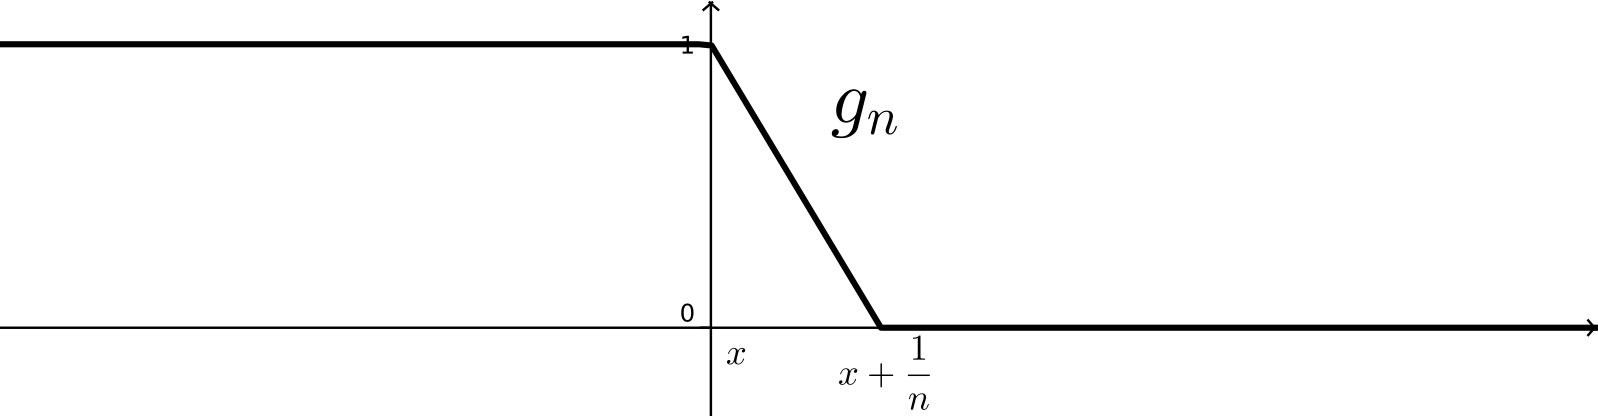
\includegraphics[width=0.5\linewidth]{veta}
				\label{fig:veta}
			\end{figure}
			
			$$(\forall k,n\in\N)\Bigl( \FF_{X_n}(x)\leq \E g_n(X_k)=\underbrace{\int\limits_{(-\infty,x]}1\dif\PP^{X_k}}_{\PP^{X_k}(-\infty,x]=\FF_{X_k}(x)}+\underbrace{\int\limits_{(x,+\infty)}(\geq 0)\dif\PP^{X_k}}_{\geq 0} \Bigr)$$
			Víme, že $X_k\Dto X$. 
			\[
			\begin{split}
			\left| \lim\limits_{ k\to +\infty} \right|:~~~~~&\liminf\limits_{ k\to +\infty} \FF_{X_k}(x)\leq \limsup\limits_{ k\to +\infty} \FF_{X_k}(x)\leq \lim\limits_{ k\to +\infty} \E g_n(X_k)=\E g_n(X)~~~\forall n\in\N \\
			\left| \lim\limits_{ n\to +\infty} \right|:~~~~~& \lim\limits_{ n\to +\infty} \E g_n(X)\equal{LDCT}\E \lim\limits_{ n\to +\infty} g_n(X)=\E \left[ 1_{(-\infty,x]}(x) \right]=\int\limits_{(-\infty,x]}1\dif\PP^X=\\
			&=\PEX\bigl( (-\infty,x] \bigr)=\FF_X(x)
			\end{split}
			\] 
			DCv: $\tilde{g}_n(t)$:
			\begin{figure}[h]
				\centering
				
\includegraphics[width=0.5\linewidth]{veta2}
				\label{fig:veta2}
			\end{figure}
			
		\end{enumerate}
	\begin{enumerate}[	$\Leftarrow$:]
	\item Volme $\epsilon>0$ a $a,b\in\tilde{D}$ tak, aby $\PP(X\in[a,b])>1-\epsilon$.
		\begin{figure}[h]
		\centering
		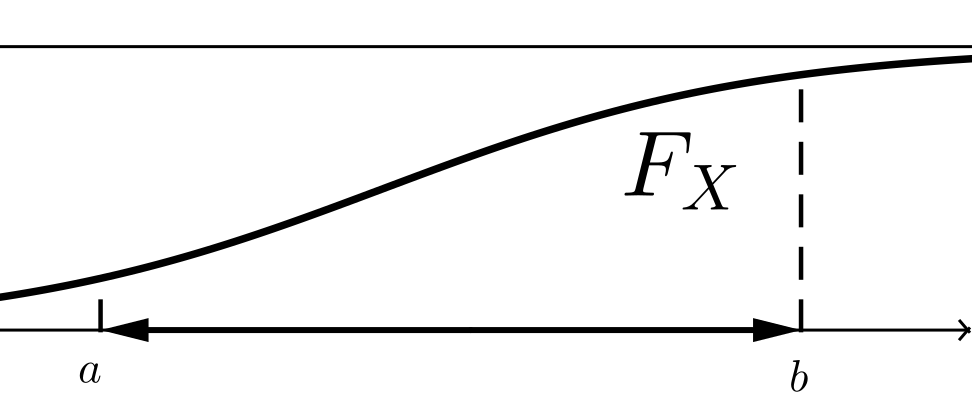
\includegraphics[width=0.3\linewidth]{veta3}
		\label{fig:veta3}
	\end{figure}
	 Volíme $g\in\CB$ libovolně fixně. Potom $g$ je stejnoměrně spojitá na $[a,b]$, tzn. $\exists a_0=a<a_1<\dots<a_k=b$ tak, že $(\forall x\in(a_j,a_{j+1}))\Bigl( \Bigl| g(x)-g(a_j) \Bigr|\leq \epsilon \Bigr)$. Definujeme dále $h(x)=\begin{cases}
	g(a_j) &\forall x\in(a_j,a_{j+1})~ \forall j \\ 0 & x<a,x>b
	\end{cases}$ a volíme $a_j\in\tilde{D}=D_X$.
	\[
	\begin{split}
	&\left| \E \left( g(X_n)-g(X) \right) \right|\leq \left| \E \left( g(X_n)-h(X_n) \right) \right|+ \left| \E \left( h(X_n)-h(X) \right) \right|+\left| \E \left( h(X)-g(X) \right) \right| \\ 
	& \left| \E \left( h(X)-g(X) \right) \right|\equal{VPI}\int\limits_{\R} \left| h(x)-g(x) \right|\dif\PP^X=\int\limits_{[a,b]}\left| h(x)-g(x) \right|\dif\PP^X+\int\limits_{[a,b]^c}\left| h(x)-g(x) \right|\dif\PP^X \leq \\ &\leq\int\limits_{[a,b]}\epsilon \dif\PP^X+\int\limits_{[a,b]^c}\underbrace{\sup|g(x)|}_{K}\dif\PP^X\leq \epsilon\cdot 1+K\int\limits_{[a,b]^c}1\dif\PP^X\leq \epsilon(1+K)  
	\end{split}
	\] 
	$$\int\limits_{[a,b]^c}1\dif\PP^X= \PP^X([a,b]^c)=\PP(X \notin [a,b])\leq \epsilon $$
	Totéž uděláme s $\left| \E \br{ g(X_n)-h(X_n)}  \right|$ a na závěr provedeme limitní přechod $n\to+\infty$.
\end{enumerate}
	\end{proof}
\end{theorem}
\begin{remark}
	Limitní věty se využívají tam, kde nejsme schopni něco vypočítat a stačí nám jistá aproximace výsledku. Máme tedy nějakou $ X\sim \PP^X $ a chceme spočítat\newline  $\PP(a<X\leq b)$.
	$$\PP(a<X\leq b)=\FF_X(b)-\FF_X(a)\equal{a,b~\in D_X}\lim \FF_{X_n}(b)-\lim \FF_{X_n}(a)\doteq \FF_{X_n}(b)-\FF_{X_n}(a)=\PP(a<X_n\leq b)$$
\end{remark}
\begin{define}
	Domluva: $\PP^{X_n}\wto \PP^X$ ozn. $X_n \Dto X$, případně $X_n\Lto X$ (podle anglického Law) a říkáme, že $X_n$ \textbf{konverguje v distribuci}.
\end{define}
\begin{remark}Opakování:
	\begin{enumerate}
		\item $X_n\Pto X \Rightarrow X_n \Dto X$
		\item $X_n \Dto c_{s.j.}\Rightarrow X_n\Pto c_{s.j.}$
	\end{enumerate}
\end{remark}
\begin{theorem}[Skorochodův reprezentační teorém]
	Mějme posloupnost náhodných veličin $\posln$ do $\R^s$, kde $X_n\Dto X$. Pak existuje $(\Omega',\Aa',\PP')$ a $(Y_n)_{n=1}^{+\infty}$ posloupnost náhodných veličin na $(\Omega',\Aa',\PP')$ takových, že $\PP^{X_n}=\PP^{Y_n}$, $\PP^X=\PP^Y$ a $Y_n\sj Y$.
	 
\end{theorem}
\begin{remark}
	\begin{enumerate}
		\item $\FF_{X_n}^{\leftarrow}\equal{\text{prosté}}\FF_{X_n}^{-1}\to \FF_{X}^{-1}$ až na spočetně mnoho výjimek.
		\item$ \lambda_{[0,1]}\bigl( \{ t:\FF_{X_n}^{\leftarrow}(t)\nrightarrow \FF_{X}^{\leftarrow}(t) \} \bigr) $, tzn. $Y_n\sj Y$
	\end{enumerate}
\end{remark}
\begin{theorem}
	Mějme $\posl$ náhodných veličin $X$ do $\R^s$ a nechť $X_n\Dto X$. Mějme $h:\R^s\to\R$ měřitelnou a spojitou $s.j.~\PP^X$. Pak $h(X_n)\Dto h(X)$.\begin{proof}
		 Skorochod: $\exists(\Omega',\Aa',\PP')$, $Y_n\sj Y$ a rozdělení zůstane zachováno, tedy 
		 $$ h\text{ spojitá }s.j.~\PP^Y~\Rightarrow~h(Y_n)\sj h(Y)~\Rightarrow~ h(Y_n)\Dto h(Y)~\Rightarrow~ h(X_n)\Dto h(X)  $$
	\end{proof}
\end{theorem}
\begin{dusl}
	Nechť $X_n\Dto X,~Y_n\Dto Y,~h:\R^2\to\R$ borelovská a spojitá $s.j.~\PP^{(X,Y)}$. Pak \textbf{neplatí}, že $(X_n,Y_n)\Dto (X,Y)$. ($\Dto$ není konvergence po složkách, takže obecně \textbf{neplatí}, že $X_n+Y_n\Dto X+Y$).
\end{dusl}
\begin{theorem}[Slutskyho perturbační teorém]
	Mějme náhodné veličiny $\posln$ do $\R^s$ tak, že $X_n\Dto X$. Nechť dále $(Y_n)_{n=1}^{+\infty}$ jsou n.v. do $\R^s$ tak, že $|X_n-Y_n|\Pto 0$. Pak $Y_n\Dto X$.\begin{proof}
		Volme $g\in\CBL$ s konstantou lipschitzovskosti $L$ a dále libovolné $\epsilon>0$. Ukážeme, že pro libovolné pevné $\epsilon>0$:
		\[
		\begin{split}
		 \bigl| \E _g(X_n)-\E _g(Y_n) \bigr|&\leq \E \bigl| g(X_n)-g(Y_n) \bigr|= \\ &=\int\limits_{|x_n-y_n|\leq\epsilon}\underbrace{\bigl| g(x_n)-g(y_n) \bigr|}_{\leq L|x_n-y_n|}\dif\PP^{(X_n,Y_n)}+\int\limits_{|x_n-y_n|>\epsilon}\underbrace{\bigl| g(x_n)-g(y_n) \bigr|}_{\leq 2\sup\limits_{x\in\R}|g(x)|}\dif\PP^{(X_n,Y_n)}\leq \\ &\leq \epsilon L+2\sup\limits_{x\in\R}|g(x)|\int\limits_{|x_n-y_n|>\epsilon}1\dif\PP^{(X_n,Y_n)}=\epsilon L+2\sup\limits_{x\in\R}|g(x)|\cdot \underbrace{\PP\Bigl( |X_n-Y_n|>\epsilon \Bigr)}_{\to 0~\forall\epsilon} 
		\end{split}
		\]
	\end{proof}
\end{theorem}
\begin{lemma}
	Nechť $X_n\Dto X$ a $Y_n\Dto c$. Pak $(X_n,Y_n)\Dto (X,c)$.
	\begin{proof}
		\begin{enumerate}[a)]
			\item $(X_n,c)\Dto (X,c)$
			\item Dosadíme do Slutskyho perturbačního teorému vektory $(X_n,Y_n)$ a $(X_n,c)$. Z a) víme, že $(X_n,c)$ konverguje. 
			$$ \bigl| (X_n,Y_n)-(X_n,c) \bigr|=\sqrt{(X_n-X_n)^2+(Y_n-c)^2}=|Y_n-c|\Pto 0 $$
		\end{enumerate}
	\end{proof}
\end{lemma}
\begin{theorem}[Slutskyho lemma]
	Nechť $X_n\Dto X$ a $Y_n\Dto c$. Pak \begin{enumerate}
		\item $X_n+Y_n\Dto X+c$
		\item $X_n\cdot Y_n\Dto X\cdot c$
		\item $X_n/Y_n\Dto X/c$,~~~ $c\neq 0$.
		
	\end{enumerate}
\end{theorem}
\begin{theorem}[Lévy continuity theorem]
	Platí několik verzí:\begin{enumerate}
		\item $X_n\Dto X \Leftrightarrow \phi_{X_n}\to \phi_X$~~~v $R^s$
		\item $\PP^{X_n}\wto \PP^X \Leftrightarrow \F(\PP^{X_n})\to \F(\PP^X)$
		\item $\F^{-1}(\PP^{X_n})\to \F^{-1}(\PP^X)\Leftrightarrow \phi_{X_n}\to \phi_X$
	\end{enumerate}
\begin{proof}[Náznak důkazu]
	\begin{enumerate}[$\Rightarrow:$]
		\item $\phi_{X_n}(t)=\E \bigl( e^{\mi tX_n} \bigr)=\E (\underbrace{\cos tX_n}_{\in\CB})+\mi \E (\underbrace{\sin tX_n}_{\in\CB})$. Díky předpokladu\newline $X_n\Dto X$ dále 
		$$ \E (\cos tX) +\mi \E (\sin tX)=\phi_X(t) $$
	\end{enumerate}
\begin{enumerate}[$\Leftarrow:$]
\item Pro $\R^1$, $a,b\in D_X$:
\[
\begin{split}
F_{X_n}(b)-\FF_{X_n}(a)&=\frac{1}{2\pi}\lim\limits_{ c\to +\infty}\int\limits_{-c}^c \frac{e^{-\mi at}-e^{-\mi bt}}{\mi t}\phi_{X_n}(t)dt \\
	\lim\limits_{ n\to +\infty} \Bigl[ \FF_{X_n}(b)-\FF_{X_n}(a) \Bigr]&\stackrel{?}{=}\frac{1}{2\pi}\lim\limits_{ c\to +\infty} \int\limits_{-c}^c \frac{e^{-iat}-e^{-ibt}}{it}\phi_{X}(t)dt=\FF_X(b)-\FF_X(a) \\
		\lim\limits_{ n\to +\infty} \FF_{X_n}(b)-\lim\limits_{ n\to +\infty} \FF_{X_n}(a) &= \FF_X(b)-\FF_X(a)
\end{split}
\] 
		Následně se zkoumá, jestli existuje $\lim\limits_{ n\to +\infty} \FF_{X_n}(b)$.
	\end{enumerate}
\end{proof}
\end{theorem}
\begin{remark}
	Říká tedy, že $\F$ i $\F^{-1}$ jsou spojité vzhledem k $\wto$.
\end{remark}
\begin{theorem}[Hélly]
	Mějme $\R^1$ a označme $\F=\{ \FF: \FF$ neklesá, je zprava spojitá a $0\leq \FF\leq 1 \}$. $\\FF_{\text{distr.~fce}}\subset\F$.\newline
	Pak $\F$ je kompaktní prostor funkcí vzhledem ke slabé limitě $\FF_n\rightarrow\FF$, tzn.\newline $(\forall \FF_n\in\F)(\exists \FF_{n_k}\in\F)\Bigl( \FF_{n_k}\rightarrow\FF \in\F \Bigr)$ na $\dom{\FF}$.
\end{theorem}
\begin{remark}
	ZVČ: $\underbrace{\oxn }_{\frac{1}{n}\suminftykn X_k}\stackrel{\PP,~s.j.}{\longrightarrow}\E  X_1=\mu\Rightarrow\oxn \Dto \mu$, tzn. $\FF_{\oxn }\to \FF_{\delta_\mu}$ (distribuční funkce Diraca).
\end{remark}
\begin{define}
	Mějme posloupnost náhodných veličin $\posln$ do $\R^1$. Říkáme, že je\textbf{ asymptoticky normální}, pokud $\exists (\mu_n)_{n=1}^{+\infty} \in\R,~\exists (\sigma_n)_{n=1}^{+\infty}>0$ tak, že 
	$$ \frac{X_n-\mu_n}{\sigma_n}\Dto Z\sim \mathrm{N}(0,1),\text{~~~ozn.~~~}X_n\sim \mathrm{AN}(\mu_n,\sigma_n^2). $$
\end{define}
\begin{remark}\begin{enumerate}
		\item $(\forall g\in\CB)\bigl( \E  g(Y_n)\to \E  g(Z) \bigr)$, a proto (pro $g(t)=t$)
		$$ \E \Bigl( \frac{X_n-\mu_n}{\sigma_n} \Bigr)=\frac{1}{\sigma_n}(\E  X_n-\mu_n)\text{~~nekonverguje k~~}\E  Z=0 $$	
		\item Praxe: $\frac{X_n-\mu_n}{\sigma_n}\Dto \mathrm{N}(0,1)~~~\Leftrightarrow~~~ \FF_{\frac{X_n-\mu_n}{\sigma_n}}\to \FF_{\mathrm{N}(0,1)}$,~~tzn.~~$\FF_{\frac{X_n-\mu_n}{\sigma_n}}\doteq \FF_{\mathrm{N}(0,1)}$, tedy $\FF_{X_n}\doteq \FF_{\mathrm{N}(\mu_n,\sigma_n^2)}$ pro dostatečně velké $n$. Z toho vyplývá, že 
		$$ P(a<X_n\leq b)=\FF_{X_n}(b)-\FF_{X_n}(a) \doteq \Phi_{\mathrm{N}(0,1)}\Bigl( \frac{b-\mu_n}{\sigma_n} \Bigr)-\Phi_{\mathrm{N}(0,1)}\Bigl( \frac{a-\mu_n}{\sigma_n} \Bigr). $$
	\end{enumerate}
\end{remark}
\begin{theorem}
	Mějme $\posln$ do $\R^1$, kde $X_n\sim \mathrm{AN}(\mu_n,\sigma_n^2)$, $\mu_n\to\mu$ a $\sigma_n^2\to 0$. Pak $X_n\Pto \mu$. $(\Rightarrow X_n\Dto \mu)$
	\begin{proof} Definujeme $Y_n:=\sigma_n~s.j.$
		$$ X_n-\mu_n=\frac{X_n-\mu_n}{\sigma_n}~Y_n\stackrel{\mathscr{D}~(Slutsky)}{\longrightarrow} \underbrace{\mathrm{N}(0,1)}_{Z}\cdot 0 = 0 \stackrel{\ref{ptocdtoc}}{\Longrightarrow}X_n-\mu_n\Pto 0\Rightarrow X_n\Pto \mu ,$$ protože $Y_n\sj 0\Rightarrow Y_n\stackrel{P,~\mathscr{D}}{\longrightarrow}0$.
	\end{proof}
\end{theorem}
\begin{theorem}[CLT (centrální limitní teorém) Lindeberg-Lévy]
	Mějme $\posl~iid~\LL_2$.\newline Pak $\oxn \sim \mathrm{AN}\Bigl(\mu,\frac{\sigma^2}{n}\Bigr)$, tzn. $\sqrt{n}~\frac{\oxn -\mu}{\sigma}\Dto \mathrm{N}(0,1)$.\newline Jiný zápis: $ \sqrt{n}~(\oxn-\mu)\Dto \mathrm{N}(0,\sigma^2) $.
	\begin{proof}
		Búno: $\mu=0,~\sigma=1$. Chceme, aby $\oxn \sim \mathrm{AN}\Bigl(0,\frac{1}{n}\Bigr)$, tzn. $\underbrace{\sqrt{n}~\oxn }_{\frac{S_n}{\sqrt{n}~}}\Dto \mathrm{N}(0,1)$.
		$$ \phi_{\frac{S_n}{\sqrt{n}~}}(t)=\phi_{\suminftykn (X_k/\sqrt{n}~)}(t)\equal{id}\prod\limits_{j=1}^n \phi_{X_j/\sqrt{n}~}(t)=\prod\limits_{j=1}^n \phi_{X_j}(\frac{t}{\sqrt{n}~})\equal{id}\Bigl[ \phi\bigl( \frac{t}{\sqrt{n}~} \bigr) \Bigr]^n\stackrel{\star}{=} $$ kde $\phi\in \mathcal{C}^{(2)}$, protože $X_k\in\LL_2$ a víme \[
			\begin{split}
			\partial_t\phi(0)=\phi'(0)&=\mi \E  X_1=0 \\
			\phi''(0)&= \mi^2\E (X_1)^2=-1\bigl( \E (X_1)^2 - (\E  X)^2 \bigr)=-\D X_1=-1 \\
			\phi(0)&=1 \\
			\phi(t)&=1-\frac{t^2}{2}+\underbrace{o(t^2)}_{\in\C}
			\end{split}
			\]
			$ \stackrel{\star}{=} \Bigl[1-\frac{t^2}{2n}+\underbrace{o\Bigl(\frac{t^2}{n}\Bigr)}_{\in\C}\Bigr]^n\longrightarrow e^{-t^2/2}=\phi_{\mathrm{N}(0,1)}(t)$\newline
			K tomu jsme využili následující fakta: $ \phi_{X_n}\to \phi_X \Leftrightarrow X_n \Dto X $~~a~~$P^X\leftrightarrow \phi_X$.\newline
			Pro libovolné $\mu$ a $\sigma$ tedy platí, že $$Y_n:=\frac{X_n-\mu}{\sigma}\Rightarrow \oyn =\frac{1}{\sigma}(\oxn -\mu)\Rightarrow \oxn  = \mu+\sigma \underbrace{\oyn}_{\Dto \mathrm{N}(0,\frac{1}{n})}\Dto N\Bigl(\mu,\frac{\sigma^2}{n}\Bigr).$$
	\end{proof}
\end{theorem}
\begin{remark}
	pro $\sigma=0$: $(\forall n\in\N)(\D\oxn=0)$, tzn. $(\forall n\in\N)(X_n\stackrel{s.j.}{=}\mu)$. 
	$$ \oxn\stackrel{s.j.}{=}\mu~\Rightarrow~\oxn\Pto\mu~\Rightarrow~\oxn\Dto \mu $$  
\end{remark}
\begin{remark}
	Měli bychom ale ověřit, že $(\star)$ platí $($ kvůli $o\Bigl(\frac{t^2}{n}\Bigr)\in\C)$.
	\[
	\begin{split}
	\Bigl[1-\frac{t^2}{2n}+o\Bigl(\frac{t^2}{n}\Bigr)\Bigr]^n&=\exp\Bigl( n \ln \bigl(1\underbrace{-\frac{t^2}{2n}+o\Bigl(\frac{t^2}{n}}_{z_n}\bigr) \Bigr)=\exp\Bigl(\frac{ n \ln \bigl(1+z_n\bigr)}{z_n}z_n \Bigr)\to \\ &\to \exp\Bigl( \lim\limits_{ n\to +\infty} n\bigl( -\frac{t^2}{2n}+o(\frac{t^2}{n}) \bigr) \Bigr)=e^{-t^2/2} 
	\end{split}
	\] 
\end{remark}
\begin{remark}
	Označíme $Z_n:=\sqrt{n}~\frac{\oxn -\mu}{\sigma}=\frac{S_n-n\mu}{\sqrt{n\sigma^2}}=\frac{S_n-\E  S_n}{\sqrt{\D  S_n}}$.
\end{remark}
\begin{theorem}[CLT Moivre-Laplace]
	Mějme $\posl~iid~\mathrm{A}(p),~p\in(0,1)$. Pak $\oxn \sim \mathrm{AN}\Bigl( p,\frac{p(1-p)}{n} \Bigr)$. \newline
	$ S_n\sim \mathrm{AN}\bigl( np,np(1-p) \bigr) $, tzn. $\frac{S_n-np}{\sqrt{np(1-p)}}\Dto \mathrm{N}(0,1)$.
\end{theorem}
\begin{remark}
	Aproximace Gaussovým rozdělením se uplatní především ke zjištění pravděpodobnosti na intervalu, kdežto pro jednotlivé body se více hodí Poisson.
\end{remark}
\begin{dusl}
	$\oxn \sim \mathrm{AN}\Bigl(\mu,\frac{\sigma^2}{n}\Bigr)$, tedy $\oxn -\mu \sim \mathrm{AN}\Bigl(0,\underbrace{\frac{\sigma^2}{n}}_{\to 0}\Bigr)\Rightarrow \oxn -\mu \Pto 0~~(o_p(1))$. Říkáme, že je konzistentní pro $\mu$. Dále\newline$n^\alpha(\oxn -\mu) \sim \mathrm{AN}\Bigl(0,\underbrace{n^{2\alpha-1}\sigma^2}_{\to 0}\Bigr)\Rightarrow n^\alpha(\oxn -\mu) \Pto 0~~~\forall \alpha<\frac{1}{2}~~(o_p(n^{-\alpha}))$. Říkáme, že je konzistentní řádu $o_p(n^{-\alpha})$ pro $\mu$.
\end{dusl}
\begin{remark}
	Pro připomenutí: značíme $\mu_j=\E X_j,~\sigma_j^2=\D X_j,~\omn=\frac{1}{n}\sum\limits_{j=1}^{n}\mu_j,$\newline$\osn=\frac{1}{n}\underbrace{\sum_{j=1}^{n}\sigma_j^2}_{B_n^2}$.
\end{remark}
\begin{theorem}[CLT Lindenberg-Feller]
	Mějme $\posl~id~\LL_2$ (nezávislé). Nechť je splněna tzv. Lindenbergova podmínka:
	$$ \mathrm{LP}_n^\epsilon =\frac{1}{B_n^2}\sum\limits_{j=1}^{n}\int\limits_{|t-\mu_j|>\epsilon B_n}|t-\mu_j|^2\dif\PP^{X_j}\stackrel{n\to+\infty}{\longrightarrow}0~~~\forall\epsilon>0~~(\text{integrujeme přes}~t) $$
	Pak $\oxn\sim \mathrm{AN}\Br{\omn,\frac{\osn}{n}}$, tzn. $S_n\sim \mathrm{AN}\Br{ \sumjn \mu_j,\sumjn \sigma_j^2}$, tedy $\frac{(\oxn-\omn)\sqrt{n}}{\sqrt{\osn}}\Dto \mathrm{N}(0,1)$.
	$$ \frac{S_n-\sum_1^n\mu_j}{\sqrt{\sum_1^n \sigma_j^2}}=\frac{S_n-\E S_n}{\sqrt{\D S_n}}\Dto \mathrm{N}(0,1) $$
	$$ \FF_{S_n}\doteq \FF_{\mathrm{N}\br{ \sum_1^n \mu_j,~\sum_1^n \sigma_j^2} } $$
\end{theorem}
\begin{remark}
	Nechť $\posl$ jsou $id~\LL_2$, $B_n\to+\infty$ a $\frac{\max\limits_{j\in\hat{n}}\sigma_j^2}{B_n^2}\to 0$. Pak\newline $(\forall\epsilon>0)(\mathrm{LP}_n^\epsilon\to 0)~\Leftrightarrow~\oxn\sim \mathrm{AN}\Br{\omn,\frac{\osn}{n}}$.
\end{remark}
\begin{theorem}[CLT$_{\nu>2}$ - Ljapunov]
	Mějme $\posl~id~\LL_{\nu>2}$. Nechť je splněna podmínka $$\mathrm{L}_j\PP_n^\nu=\sumjn \E|X_j-\mu_j|^\nu=o\br{B_n^\nu},~\text{tzn}~~~\frac{\sum_1^n \E|X_j-\mu_j|^\nu}{B_n^\nu}\stackrel{n\to+\infty}{\longrightarrow}0.$$
	Pak $\oxn\sim \mathrm{AN}\Br{\omn,\frac{\osn}{n}}$.
	\begin{proof}Platí odhad
		$$ 1<\frac{|t-\mu_j|}{\epsilon B_n}<\frac{(t-\mu_j)^2}{\epsilon^2 B_n^2}<\frac{|t-\mu_j|^\nu}{\epsilon^\nu B_n^\nu} $$
		\[
		\begin{split}
		\mathrm{LP}_n^\epsilon&=\frac{1}{B_n^2}\sumjn \int\limits_{|t-\mu_j|>\epsilon B_n}|t-\mu_j|^2\dif\PP^{X_j}\leq \frac{1}{B_n^2}\sumjn \int\limits_{|t-\mu_j|>\epsilon B_n}|t-\mu_j|^\nu \epsilon^{2-\nu}B_n^{2-\nu} \dif\PP^{X_j}\leq \\ &\leq \epsilon^{2-\nu}B_n^{-\nu}\sumjn \int\limits_{\R} |t-\mu_j|^\nu \dif\PP^{X_j}=\epsilon^{2-\nu}\frac{\sum_1^n \E|X_j-\mu_j|^\nu}{B_n^\nu}\stackrel{\forall\epsilon>0}{\longrightarrow}0
		\end{split}
		\]
	\end{proof}
\end{theorem}
\begin{theorem}[Pólya theorem]
	Mějme náhodné veličiny $\posl,~X$ a distribuční funkce $(\FF_{X_j})_{j=1}^{+\infty},~\FF_X$. Nechť $\FF_{X_j}\to \FF_X$ a $\FF_X$ je spojitá. Pak $\FF_{X_j}\stackrel{\R}{\rightrightarrows}\FF_X$.
\end{theorem}
\begin{dusl}
	Konvergence v $CLT$ je stejnoměrná na $\R$.
	$$ \sup\limits_{x\in\R}\bigl| \FF_{Z_n}-\FF_{\mathrm{N}(0,1)} \bigr|\stackrel{n\to+\infty}{\longrightarrow} 0,~~\text{kde }Z_n:=\frac{S_n-\E S_n}{\sqrt{\D S_n}} $$
\end{dusl}
\begin{theorem}[Berry-Essen]
	Nechť $\posl~iid~\LL_3$. Pak
	$$ \sup\limits_{x\in\R}\bigl| \FF_{Z_n}-\FF_{\mathrm{N}(0,1)} \bigr|\leq c~\frac{\E |X_1-\mu|^3}{\sigma^3}\frac{1}{\sqrt{n}}=O(\frac{1}{\sqrt{n}}), $$ kde $c$ je konstanta menší než 1.
\end{theorem}


\begin{theorem}
	Mějme $(\X_j)_{j=1}^{+\infty}~iid~\LL_2$ do $\R^s$. Označme $\boldsymbol\mu=\E\X_j,~\C=\Cov(\X_j)$~~$\forall j\in\N$. Definujeme $Y_j=\boldsymbol\alpha(\X_j-\boldsymbol\mu)~~\forall\boldsymbol\alpha\in\R^s$.
	$$ \E Y_j=\boldsymbol\alpha(\E\X_j-\boldsymbol\mu)=0 $$
	$$ \D Y_j = \D \br{\boldsymbol\alpha(\X_j-\boldsymbol\mu)}=\D(\boldsymbol\alpha\X_j)=\boldsymbol\alpha\C\boldsymbol\alpha^T<+\infty $$
	
\end{theorem}
\begin{remark}
	Mějme $Y_j~iid~\LL_2$ $(\mu=0,~\sigma^2=\boldsymbol\alpha\C\boldsymbol\alpha^T)$. Pak podle CLT$_{L-L}$ v $\R^1$ platí \[
	\begin{split}
	\sqrt{n}~(\oyn-0)&\Dto \mathrm{N}\br{0,\boldsymbol\alpha\C\boldsymbol\alpha^T}\\
	\boldsymbol\alpha\sqrt{n}~(\oxn-\boldsymbol\mu)&\Dto \mathrm{N}\br{0,\boldsymbol\alpha\C\boldsymbol\alpha^T}\\
	\boldsymbol\alpha\mathbb{U}_n&\Dto \mathrm{N}\br{0,\boldsymbol\alpha\C\boldsymbol\alpha^T},~~\text{kde }\mathbb{U}_n=\sqrt{n}~(\oxn-\boldsymbol\mu),
	\end{split}
	\] kde $\C$ je kovariantní maticí $\mathbb{U}$.
	$$ \forall\boldsymbol{\alpha}\in\R^s:~\boldsymbol{\alpha}\mathbb{U}_n\Dto \boldsymbol{\alpha}\mathbb{U}~~\Rightarrow~~\mathbb{U}_n\Dto \mathbb{U}, $$ kde $\mathbb{U}$ má takové rozdělení, že $\boldsymbol{\alpha}\mathbb{U}\sim \mathrm{N}_1(0,\boldsymbol{\alpha}\C\boldsymbol{\alpha}^T)$, tedy $\D(\boldsymbol{\alpha}\mathbb{U})=\boldsymbol{\alpha}\Cov(\mathbb{U})\boldsymbol{\alpha}^T$.
\end{remark}
\begin{define}
	Mějme $(\X)_{j=1}^{+\infty}$ do $\R^s$. Řekneme, že mají \textbf{s-rozměrné Gaussovo rozdělení}, pokud 
	$$ \boldsymbol{\alpha}\X\sim \mathrm{N}_1\br{\boldsymbol{\alpha}\boldsymbol{\mu},\boldsymbol{\alpha}\C\boldsymbol{\alpha}^T }~~~\forall\boldsymbol{\alpha}\in\R^s, $$ kde označujeme $\boldsymbol{\mu}=\E\X$ a $\C=\Cov(\X)$.
\end{define}
\begin{theorem}[CLT v $\R^s$]
	Mějme $(\X_j)_{j=1}^{+\infty}~iid~\LL_2$ (do $\R^s$). Pak $\oxn\sim \mathrm{AN}_s\br{\boldsymbol{\mu},\frac{1}{n}\C}$.
\end{theorem}
\begin{remark}
	Mějme $\oxn\sim\mathrm{AN}\br{\mu,\frac{\sigma^2}{n}}$, tzn. $\FF_{\oxn}\cdot \FF_{\mathrm{N}(\mu,\frac{\sigma^2}{2})}$. Zajímá nás, jestli platí vztah $\FF_{\oxn^2}\cdot \FF_{[\mathrm{N}(\mu,\frac{\sigma^2}{2})]^2}$.
		$$ \sqrt{n}~\br{\frac{\oxn-\mu}{\sigma}}\Dto \mathrm{N}(0,1) $$
		$$ g(T)=t^2 \text{ spojitá }\Rightarrow \left[ \br{\frac{\oxn-\mu}{\sigma}} \right]^2 \Dto [\mathrm{N}(0,1)]^2=\chi^2(1) $$
\end{remark}
\begin{theorem}[Delta-metoda $(\nabla)$]
	Mějme $(\X_n)_{n=1}^{+\infty}$ do $\R^s$, $\X_n\sim\mathrm{AN}_s(\boldsymbol{\mu}_n,\sigma_n^2\C)$. Nechť dále $\mu_n\to\mu,~\sigma_n\to 0$ a $g:\R^s\to\R^1$ je borelovská spojitě diferencovatelná funkce. Pak 
	$$ g(\X_n)\sim\mathrm{AN}\br{g(\boldsymbol{\mu}_n),\sigma_n^2\nabla g(\boldsymbol{\mu})\C\nabla g(\boldsymbol{\mu})^T}. $$
	\begin{proof}
		Rozvoj Taylorovy řady $\forall n\in\N$:
		$$ g(\X_n)=g(\boldsymbol{\mu}_n)+\underbrace{g'(\xi_n)}_{\nabla g(\xi_n)}(\X_n-\boldsymbol{\mu}_n), $$
		kde $\xi_n$ leží na spojnici $\boldsymbol{\mu}_n$ a $\X_n$, tzn. $\xi_n=\xi_n(\X_n)$. Víme, že $\X_n\Pto \boldsymbol{\mu}$ a $\boldsymbol{\mu}_n\to\boldsymbol{\mu}$. Z toho vyplývá, že $\xi_n\Pto \bmu~~\Rightarrow~~ g'(\xi_n)\Pto g'(\bmu)$.
		$$ \frac{g(\X_n)-g(\bmu_n)}{\sigma_n}=\underbrace{g'(\xi_n)}_{\Pto g'(\bmu)}\underbrace{\frac{\X_n-\bmu_n}{\sigma_n}}_{\Dto \mathrm{N}_s(\textbf{0},\C)} \stackrel{\mathscr{D}~\text{(Slutsky)}}{\longrightarrow}\underbrace{g'(\bmu)}_{\nabla g(\bmu)}\mathrm{N}_s(\textbf{0},\C)=\mathrm{N}_1(0,\nabla g(\bmu)\C\nabla g(\bmu)^T. $$
	\end{proof}
\end{theorem}
\begin{theorem}
	Mějme $\X\sim \mathrm{N}_s(\bmu,\C)$. Pak $\phi_\X(\textbf{t})=e^{\mi \bmu\textbf{t}-\frac{1}{2}\textbf{t}\C\textbf{t}^T}~~~\forall \textbf{t}\in\R^s$.
	\begin{proof}
		Důkaz ponechán čtenáři. Nápověda: použít $Y=\textbf{t}\X\sim\mathrm{N}_1(\textbf{t}\bmu,\textbf{t}\C\textbf{t}^T)$.
	\end{proof}
\end{theorem}
\begin{theorem}
	Nechť $\X\sim\mathrm{N}_s(\bmu,\C)$, $\mathbb{D}$ je matice $s\cdot k,~1\leq k\leq s$. Pak $\mathbb{Y}=\mathbb{D}\X\sim \mathrm{N_k(\mathbb{D}\bmu,\mathbb{D}\C\mathbb{D}^T)}$.\begin{proof}
		$$ \phi_{\mathbb{Y}}(\textbf{t})=\phi_{\mathbb{X}}(\textbf{t}\mathbb{D})=e^{\mi \bmu\textbf{t}\mathbb{D}-\frac{1}{2}\textbf{t}\mathbb{D}\C(\textbf{t}\mathbb{D})^T} \sim \mathrm{N}_k(\mathbb{D}\bmu,\mathbb{D}\C\mathbb{D}^T)$$
	\end{proof}
\end{theorem}
\begin{theorem}
	Nechť $\X\sim \mathrm{N}_1(\bmu,\C)$. Pak $X_j$ jsou nezávislé $\Leftrightarrow~(X_j)_1^s$ jsou po dvou nekorelované.
	\begin{proof}
		\begin{enumerate}[$\Rightarrow$:]
			\item Zřejmé z definice.
		\end{enumerate}
	\begin{enumerate}[$\Leftarrow$:]
	\item Stačí ukázat, že $\phi_\X=\prod\limits_{j=1}^s \phi_{X_j}(t_j)$.
\end{enumerate}
	\end{proof} 
\end{theorem}
\begin{dusl}
	$(X_j)_1^s~id~\mathrm{N}(\mu_j,\sigma_j^2)~\Leftrightarrow~\X\sim\mathrm{N}_s(\bmu,\C=\diag(\sigma_j^2)_1^s)$
\end{dusl}
\begin{theorem}
	Mějme $\X\sim\mathrm{N}_s(\bmu,\C)$ a nechť $\C$ je regulární (tzn. $\C$ je PD). Pak $\exists\mathbb{A}$ regulární ($s\cdot s$) tak, že $\X=\mathbb{A}\mathbb{Z}+\bmu$, kde $\mathbb{Z}\sim\mathrm{N}_s(\textbf{0},\mathbb{I})$ a $\mathbb{A}\mathbb{A}^T=\C$. ($(Z_j)_1^s~iid~\mathrm{N}(0,1)$)
\end{theorem}
\begin{theorem}
	Mějme $\X\sim\mathrm{N}_s(\bmu,\C)$. Pak hustota pravděpodobnosti $\X$ existuje $\Leftrightarrow~\C$ je regulární.
	$$ f_\X(\textbf{x})=\frac{1}{(\sqrt{2\pi})^n\sqrt{|\C|}}e^{-\frac{1}{2}(\textbf{x}-\bmu)^T\C^{-1}(\textbf{x}-\bmu)} $$ 
\end{theorem}